\chapter{\LaTeX 示例}
\section{公式}
\begin{equation}
\vec{P}_{i}(u)=\sum_{j=0}^{k} \vec{V}_{i} \Lambda_{i}\left(k ; \vec{\beta}_{1}, \cdots \vec{\beta}_{n} ; u\right)
\end{equation}

\begin{equation}
\frac{|A(s)|^{2}}{|A(o)|^{2}}=\frac{\rho_{1} \rho_{2}}{\left(s+\rho_{1}\right)\left(s+\rho_{2}\right)}
\end{equation}

\section{表格}

\begin{table}[h]
\centering
\caption{压降损失计算结果}
\label{table:jiangya}
\begin{tabularx}{\textwidth}{CCC}
\toprule[2pt]
换热器&热边压降损失&冷边压降损失\\
\midrule[1pt]
初级&2974.37&2931.52\\
次级&2924.65&3789.76\\
\bottomrule[2pt]
\end{tabularx}
\end{table}

\section{图}


\begin{figure}[!h]
\centering
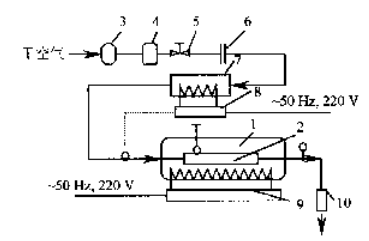
\includegraphics[width=0.5\textwidth]{figures/danguan}\\
\footnotesize
1-太阳模拟器;2-单管及 31 个 PCM 容器;3-气泵;\\
4-干燥过滤器;5-手动调节阀;6-孔板流量计;\\
7-空气预热器;8,9-调功器;10-空气换热器.\\
\caption{单管换热系统流程图}
\label{fig:danguan}
\end{figure}


\begin{figure}[!h]
  \subfigure[t][分布符合 $1 / f$ 规律图]{
    
\includegraphics[width=0.25\textwidth]{figures/a}
  }
  \hfill
  \subfigure[t][大小与色彩符合 $1 / f$ 规律图]{
    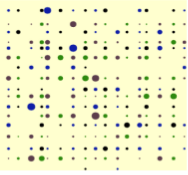
\includegraphics[width=0.25\textwidth]{figures/b}
  }
  \hfill
  \subfigure[t][间距、大小与色彩均符合 $1 / f$ 规律图]{
    
\includegraphics[width=0.25\textwidth]{figures/c}
  }
  \caption{图案例}
  \label{fig:tuan}
\end{figure}


